\chapter{Electric / Hybrid RV Propulsion}
\section{Introduction}
\subsection{Reasons forcing change}
\begin{itemize}
    \item Global warming e.g. CO2 emissions
    \item Health e.g. NOx emissions
    \item Efficiency e.g. low efficiency of vehicles presently
    \item Technology advances e.g. batteries
    \item Increasing demand e.g. in developing countries
    \item Custom demand e.g. environmental concerns
\end{itemize}
\subsection{Global CO2 emissions}
\begin{figure}[H]
    \centering
    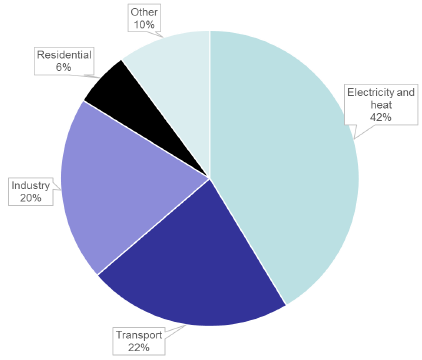
\includegraphics[width = 0.8\textwidth]{img/figure92.png}
    \caption{Global CO2 emissions.}
\end{figure}
Transport is a significant contribution to CO2 global emissions. It is a bigger emitter than electricity generation in many countries.
\subsection{Typical driving energy losses (city use)}
\begin{figure}[H]
    \centering
    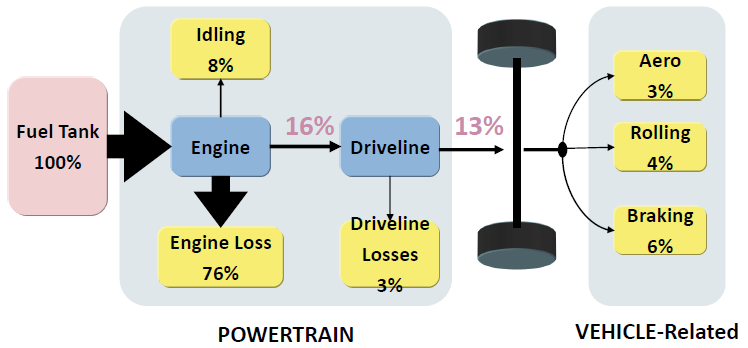
\includegraphics[width = 0.8\textwidth]{img/figure93.png}
    \caption{Typical driving energy losses (city use).}
\end{figure}
The efficiency of ICE engines in road vehicles is low.
\subsection{Transport sector growth prediction}
\begin{figure}[H]
    \centering
    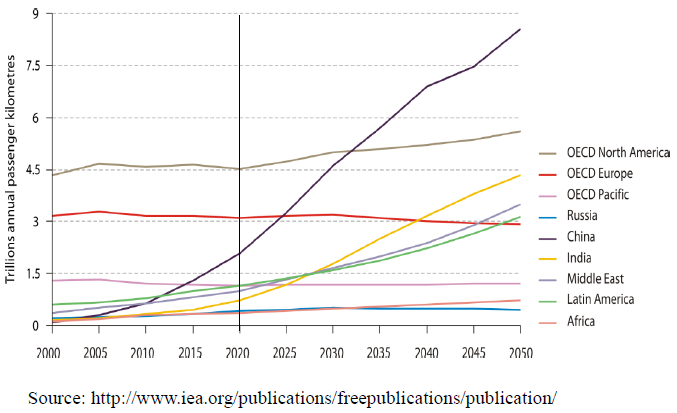
\includegraphics[width = 0.8\textwidth]{img/figure94.png}
    \caption{Transport sector growth prediction.}
\end{figure}
Transport growth is mainly in developing countries whereas developed countries are expected to remain unchanged.
\subsection{Gasoline: the (almost) perfect fuel}
\begin{figure}[H]
    \centering
    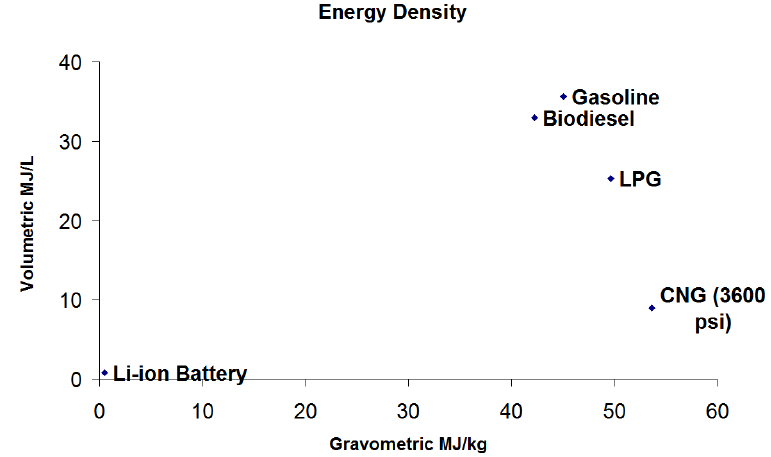
\includegraphics[width = 0.8\textwidth]{img/figure95.png}
    \caption{Transport sector growth prediction.}
\end{figure}
\subsection{Towards zero emissions}
\begin{figure}[H]
    \centering
    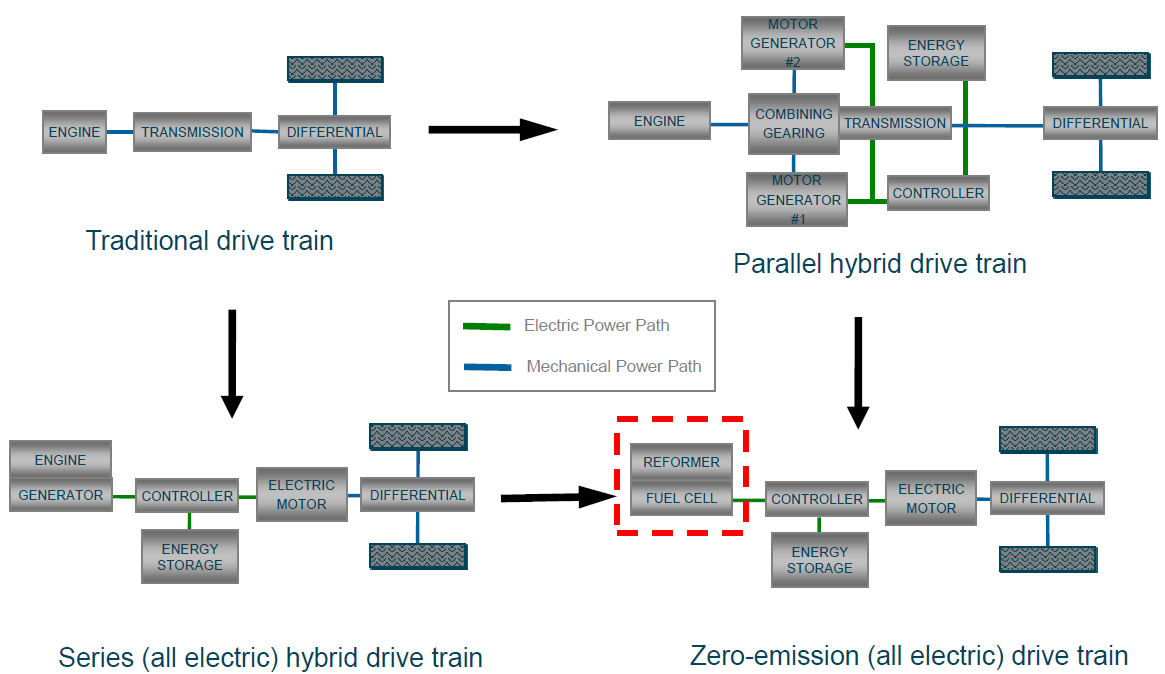
\includegraphics[width = 0.8\textwidth]{img/figure96.png}
    \caption{Drive trains for various vehicle types.}
\end{figure}
